\documentclass[12pt]{article}
%% \usepackage[top=1in,left=1.25in, right = 1.25in, bottom=1in]{geometry}

\usepackage{graphicx}
\usepackage{xspace}
%\usepackage{adjustbox}

\usepackage{afterpage}

\usepackage{grffile}

\newcommand{\comment}{\showcomment}
%% \newcommand{\comment}{\nocomment}

\newcommand{\showcomment}[3]{\textcolor{#1}{\textbf{[#2: }\textsl{#3}\textbf{]}}}
\newcommand{\nocomment}[3]{}

\newcommand{\jd}[1]{\comment{cyan}{JD}{#1}}
\newcommand{\swp}[1]{\comment{magenta}{SWP}{#1}}
\newcommand{\bmb}[1]{\comment{blue}{BMB}{#1}}
\newcommand{\djde}[1]{\comment{red}{DJDE}{#1}}

\newcommand{\eref}[1]{Eq.~\ref{eq:#1}}
\newcommand{\fref}[1]{Fig.~\ref{fig:#1}}
\newcommand{\Fref}[1]{Fig.~\ref{fig:#1}}
\newcommand{\sref}[1]{Sec.~\ref{#1}}
\newcommand{\frange}[2]{Fig.~\ref{fig:#1}--\ref{fig:#2}}
\newcommand{\tref}[1]{Table~\ref{tab:#1}}
\newcommand{\tlab}[1]{\label{tab:#1}}
\newcommand{\pday}{\ensuremath{/\textrm{day}}}

\usepackage{amsthm}
\usepackage{amsmath}
\usepackage{amssymb}
\usepackage{amsfonts}

\usepackage{lineno}
\linenumbers

\usepackage[pdfencoding=auto, psdextra]{hyperref}

\usepackage{natbib}
\bibliographystyle{chicago}
\date{\today}

\usepackage{xspace}
\newcommand*{\ie}{i.e.\@\xspace}

\usepackage{color}

\newcommand{\Rx}[1]{\ensuremath{{\mathcal R}_{#1}}\xspace} 
\newcommand{\Ro}{\Rx{0}}
\newcommand{\Rc}{\Rx{\mathrm{c}}}
\newcommand{\Ri}{\Rx{\mathrm{i}}}
\newcommand{\RR}{\ensuremath{{\mathcal R}}\xspace}
\newcommand{\Rhat}{\ensuremath{{\hat\RR}}}
\newcommand{\Rprop}{\Rx{\mathrm{prop}}}
\newcommand{\Rcori}{\Rx{\mathrm{cori}}}
\newcommand{\tsub}[2]{#1_{{\textrm{\tiny #2}}}}
\newcommand{\dd}[1]{\ensuremath{\, \mathrm{d}#1}}
\newcommand{\dtau}{\dd{\tau}}
\newcommand{\dx}{\dd{x}}
\newcommand{\dsigma}{\dd{\sigma}}

\newcommand{\tstart}{\ensuremath{\tsub{t}{start}}\xspace}
\newcommand{\tend}{\ensuremath{\tsub{t}{end}}\xspace}

\newcommand{\betaeff}{\ensuremath{\tsub{\beta}{eff}}\xspace}
\newcommand{\Keff}{\ensuremath{\tsub{K}{eff}}\xspace}
\newcommand{\Kpost}{\ensuremath{\tsub{K}{post}}\xspace}

\newcommand{\pt}{p} %% primary time
\newcommand{\st}{s} %% secondary time

\newcommand{\psize}{{\mathcal P}} %% primary cohort size
\newcommand{\ssize}{{\mathcal S}} %% secondary cohort size

\newcommand{\gtime}{\sigma} %% generation interval
\newcommand{\gdist}{g} %% generation-interval distribution

\newcommand{\geff}{g_{\textrm{eff}}} %% generation-interval distribution

\newcommand{\total}{{\mathcal T}} %% total number of serial intervals

\newcommand{\PP}{\ensuremath{\mathcal P}}
\newcommand{\II}{\ensuremath{\mathcal I}}
\newcommand{\HH}{\ensuremath{\mathcal H}}
\newcommand{\VE}{\ensuremath{\mathrm{VE}}}
\newcommand{\VEP}{\ensuremath{\VE_{\mathrm{P}}}}
\newcommand{\VEL}{\ensuremath{\VE_{\mathrm{L}}}}

\begin{document}

\begin{flushleft}{
	\Large
	\textbf\newline{
		Immune boosting bridges leaky and polarized vaccination models
	}
}
\newline
\\
Sang Woo Park\textsuperscript{1,*}, Michael Li, Chadi Saad-Roy, ???, Bryan T Grenfell, Jonathan Dushoff
\\
\bigskip
\textbf{1} Department of Ecology and Evolutionary Biology, Princeton University, Princeton, NJ, USA
\\
\bigskip

*Corresponding author: swp2@princeton.edu
\end{flushleft}

\section*{Introduction}

Vaccination plays a critical role in controlling infectious disease outbreaks by protecting against new infections \citep{iwasaki2020and}.
In particular, when a critical vaccination threshold is reached, the basic reproduction number (defined as the average number of secondary infections caused by an infected individual) is reduced to below 1, and future epidemics can be prevented \citep{anderson1985vaccination}.
But reaching a critical vaccination threshold can be challenging, and vaccines often provide imperfect protections \citep{gandon2003imperfect,anderson2020challenges}.

There are two main ways of modeling vaccines with imperfect protections: ``leaky'' and ``all-or-nothing'' vaccine \citep{smith1984assessment}.
The leaky vaccination model assumes that vaccinated individuals experience a reduced force of infection (e.g., multiplied by a factor $1-\VEL < 1$).
The ``all-or-nothing'' vaccination model assumes that the proportion \VEP\ of vaccinated individuals are completely protected and the remaining proportion $1-\VEP$ of vaccinated individuals are completely susceptible.
This model is analogous to the polarized immunity model, in which infection from one strain gives complete or no protection against other strains \citep{gog2002dynamics}---we thus refer to this model as the polarized vaccination model \citep{gomes2014missing}.
Here, both \VEL\ and \VEP\ represent vaccine efficacy, which we define as the proportion of people protected from their first challenge.

When these two models are used with the same nominal vaccine efficacy $\VEL = \VEP$, they predict different epidemic dynamics, including the final size \citep{smith1984assessment}:
for high force of infection, almost all individuals eventually get infected in the leaky model, whereas many individuals are permanently protected in the polarized model.
Modelers tend to rely on the leaky assumption, including throughout the SARS-CoV-2 pandemic \citep{dyson2021possible,gozzi2021importance,marziano2021vaccine,matrajt2021vaccine,park2022intermediate} with some exceptions \citep{bubar2021model,buckner2021dynamic}.
Various reasons have been given, but most likely is a combination of convenience and tradition.

Both models represent simplifications of reality.
The leaky model in particular overlooks a potentially important mechanism: individuals in this model do not lose any susceptibility when (implicitly) exposed to a challenge that does not result in infection. 
In fact, vaccinated individuals who successfully fight off exposures can experience immune boosting, thus becoming less susceptible to future infections without becoming infectious or developing symptoms from the exposure \citep{lavine2011natural,yang2020waning}.

In this study, we compare different approaches to dynamical modeling of vaccination and immunity.
First, we construct a model with leaky vaccination and boosting, and show that the transmission dynamics of this model can bridge from the dynamics of the standard leaky model (with no boosting) to those of the polarized model (with perfect boosting). 
%% In doing so, we show that the polarized vaccination and immune boosting models predict identical epidemic dynamics but different serological dynamics.
Then, we construct a generalized vaccination model, which includes all three mechanisms, and explore its dynamics.
Finally, we use our framework to compare measures of vaccine efficacy.

\section*{Mathematical models of vaccine-induced immunity}

\afterpage{
\begin{figure}[!th]
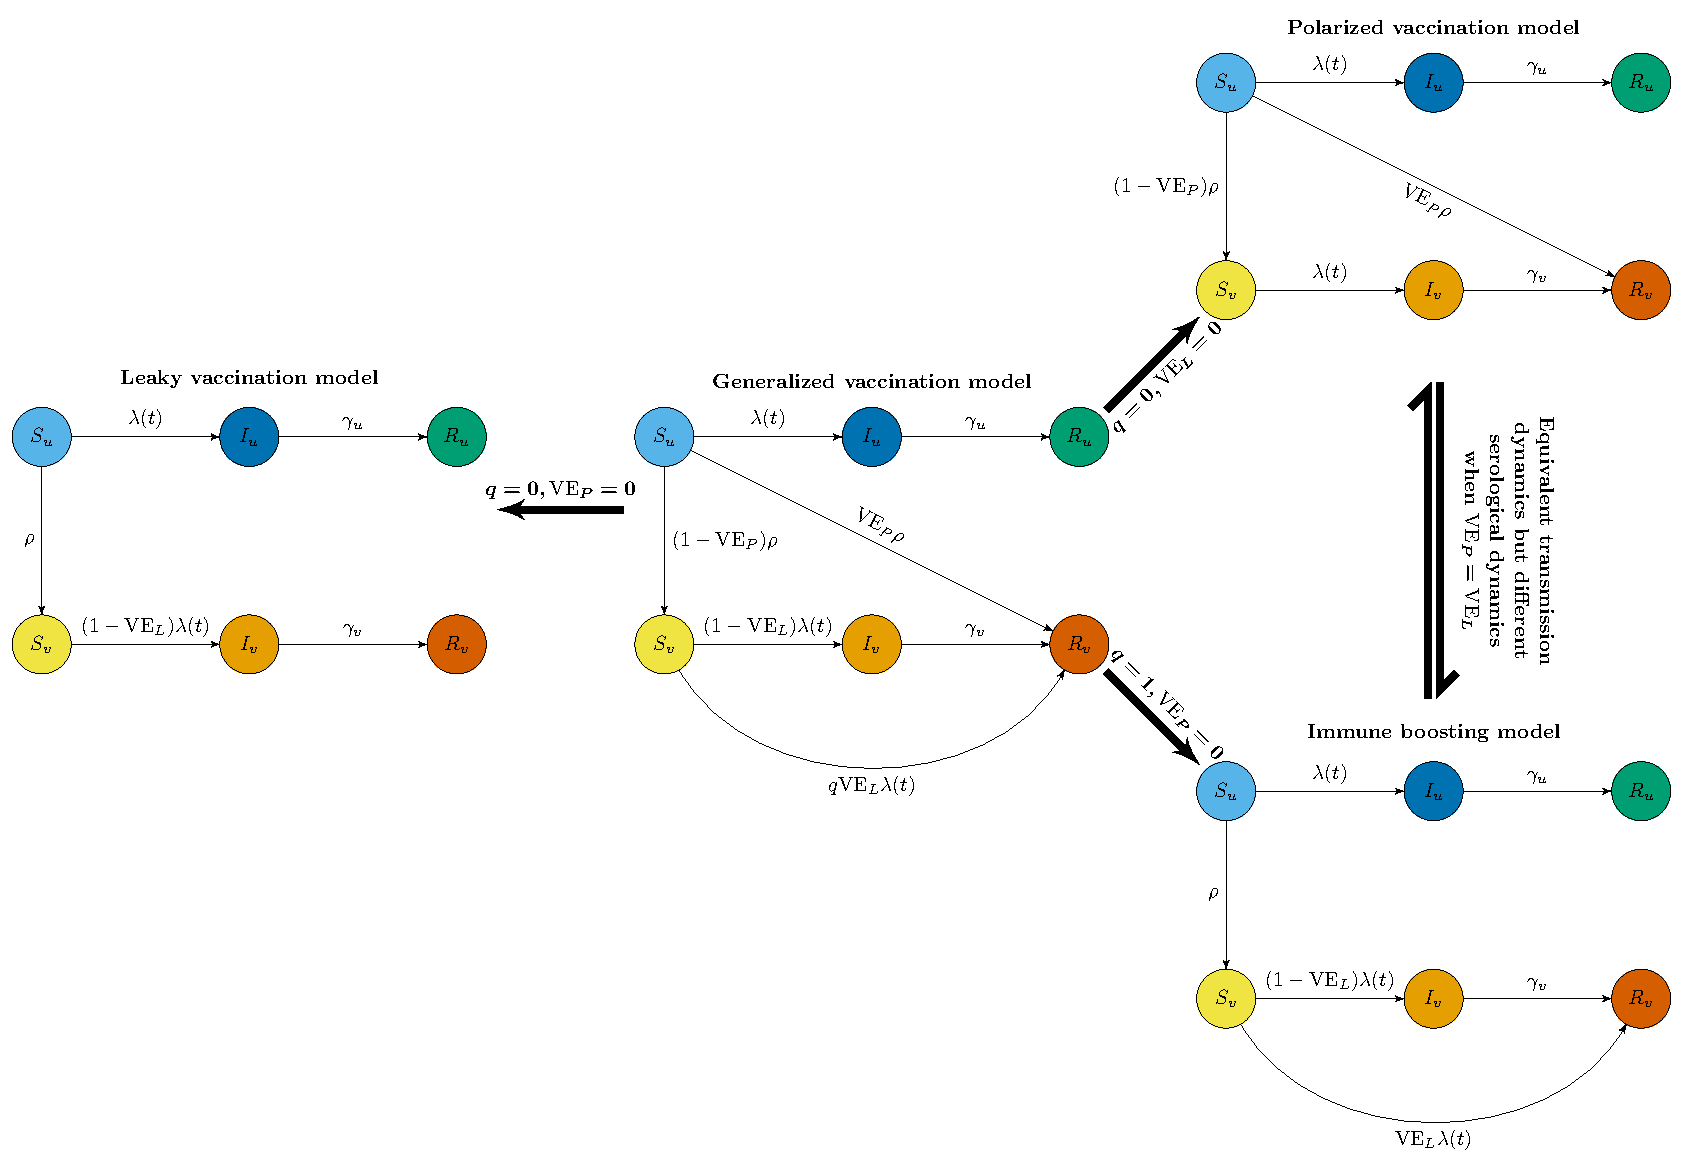
\includegraphics[width=\textwidth]{figure_diagram_comb.pdf}
\caption{
\textbf{A schematic diagram of vaccination models.}
$S$ represents susceptible individuals. $I$ represents infected individuals. $R$ represents recovered individuals.
$\lambda$ represents force of infection. 
$p$ represents vaccine efficacy.
$\gamma$ represents recovery rate.
$\theta$ represents the proportion of individuals that remain partially susceptible after vaccination.
$q$ represents the proportion of unsuccessful challenges that result in immune boosting.
Subscripts $u$ and $v$ represents unvaccinated and vaccinated.
\label{fig:diagram}
}
\end{figure}
}

Throughout the paper, we assume that a population mixes homogeneously and that there is no loss of immunity.
We begin with a standard SIR model with a leaky vaccine, in which all vaccinated individuals experience a reduced force of infection by a factor of $1-\VEL$:
\begin{align}
\frac{\dd S_u}{\dd t} &= - \lambda(t) S_u - \rho S_u \\
\frac{\dd I_u}{\dd t} &= \lambda(t) S_u - \gamma_u I_u \\
\frac{\dd R_u}{\dd t} &= \gamma_u I_u \\
\frac{\dd S_v}{\dd t} &= - (1-\VEL) \lambda(t) S_v + \rho S_u \\
\frac{\dd I_v}{\dd t} &= (1-\VEL) \lambda(t) S_v - \gamma_v I_v \\
\frac{\dd R_v}{\dd t} &= \gamma_v I_v
\end{align}
where subscripts $u$ and $v$ indicate the unvaccinated and vaccinated individuals;
$\lambda$ represents the baseline force of infection experienced by unvaccinated individuals; 
$\rho$ represents vaccination rate;
$\gamma$ represents the recovery rate;
and \VEL\ represents the vaccine efficacy, which also captures the amount of reduction in the probability of infection.
This kind of model is sometimes called “history-based”, since susceptibility of an individual depends only on their history of infections (or vaccination) \citep{gog2002dynamics,gog2002status,kucharski2016capturing}.

Conversely, the polarized vaccination model assumes that a proportion \VEP\ of vaccinated individuals become fully immune, whereas the remaining proportion $1-\VEP$ remain susceptible: 
\begin{align}
\frac{\dd S_u}{\dd t} &= - \lambda(t) S_u - \rho S_u \\
\frac{\dd I_u}{\dd t} &= \lambda(t) S_u - \gamma_u I_u \\
\frac{\dd R_u}{\dd t} &= \gamma_u I_u \\
\frac{\dd S_v}{\dd t} &= - \lambda(t) S_v + (1-\VEP) \rho S_u \\
\frac{\dd I_v}{\dd t} &= \lambda(t) S_v - \gamma_v I_v \\
\frac{\dd R_v}{\dd t} &= \gamma_v I_v + \VEP \rho S_u
\end{align}
This is the approach used in “status-based” models of cross immunity---such models keep track of immune statuses of individuals, rather than their infection histories \citep{gog2002dynamics,gog2002status,kucharski2016capturing}.
For this model, the parameter \VEP\ is the measure of vaccine efficacy.

These two widely used models have important dynamical differences. For a given set of shared parameters, and the same value of vaccine efficacy, initial dynamics will be the same, but the permanent protection of individuals in the polarized model will always result in a lower final outbreak size than the leaky vaccination model. When both \VE\ and the initial value of \Rx\ are relatively high, this difference is large.

To better understand this gap, we consider a immune boosting model.
The leaky vaccination model assumes that vaccinated individuals are challenged with a lower force of infection $(1-\VEL) \lambda(t)$, but in general it is not realistic to assume that challenges would completely disappear only because of immune status.
In a homogeneously mixing population, we expect both vaccinated and unvaccinated individuals to be challenged with identical forces of infection $\lambda$.
Therefore, the leaky vaccination model implicitly assumes that vaccinated individuals have an \emph{independent} probability $(1-\VEL)$ of infection for every challenge.
Instead, the immune boosting model assumes that unsuccessful challenges elicit immune response, moving individuals from $S_v$ to $R_v$ compartment at rate $\VEL \lambda(t)$ and thereby breaking the independence assumption of the leaky vaccine model:  
\begin{align}
\frac{\dd S_u}{\dd t} &= - \lambda(t) S_u - \rho S_u \\
\frac{\dd I_u}{\dd t} &= \lambda(t) S_u - \gamma_u I_u \\
\frac{\dd R_u}{\dd t} &= \gamma_u I_u \\
\frac{\dd S_v}{\dd t} &= - \lambda(t) S_v + \rho S_u \\
\frac{\dd I_v}{\dd t} &= (1-\VEL) \lambda(t) S_v - \gamma_v I_v \\
\frac{\dd R_v}{\dd t} &= \VEL \lambda(t) S_v + \gamma_v I_v
\end{align}
In this model, both unvaccinated and vaccinated individuals are subject to identical forces of infection, which represent the per capita rate of challenges, but the outcome of challenges differ.

The epidemiological dynamics (i.e., trajectories of $I_u$ and $I_v$) predicted by the immune-boosting model (based on leaky vaccination) and the polarized vaccination model are identical: 
both models assume that individuals become vaccinated at rate $\rho$ and move out of the $S_v$ compartment at rate $\lambda$ and only differ in when individuals get sorted based on the result of their next challenge.
This equivalence allows us to bridge the difference between the leaky and polarized vaccination models.
The equivalence holds regardless of infection characteristics of vaccinated individuals (i.e., the duration of their infection and their transmissibility);
however, it may not necessarily hold when immunity wanes, as we discuss later.

Finally, we consider a generalized model that encompasses all three mechanisms above (dichotomous vaccine responses, partial protection, and immune boosting):
\begin{align}
\frac{\dd S_u}{\dd t} &= - \lambda(t) S_u - \rho S_u \\
\frac{\dd I_u}{\dd t} &= \lambda(t) S_u - \gamma_u I_u \\
\frac{\dd R_u}{\dd t} &= \gamma_u I_u \\
\frac{\dd S_v}{\dd t} &= - [1- (1-q) \VEL] \lambda(t) S_v + (1-\VEP) \rho S_u \\
\frac{\dd I_v}{\dd t} &= (1-\VEL) \lambda(t) S_v - \gamma_v I_v \\
\frac{\dd R_v}{\dd t} &= \VEP \rho S_u + q \VEL \lambda(t) S_v + \gamma_v I_v
\end{align}
This model includes one new parameter, $q$, which represents the proportion of unsuccessful challenges that result in immune boosting.
When $q=0$ (i.e., in the absence of boosting), setting $\VEP = 0$ gives us the leaky vaccination model. 
When $q=1$ (i.e., in the presence of full boosting), setting $\VEP = 0$ gives us the immune boosting model, whereas setting $\VEL = 0$ gives us the polarized vaccination model. 
The relationship between these four models are summarized in \fref{diagram}.

We note that the generalized vaccination model has a combined vaccine efficacy of $\VE = 1- (1-\VEL) (1-\VEP)$, and therefore always has higher efficacy than any of the individual models.
Therefore, we later analyze the dynamics of the generalized vaccination model while keeping $\VE$ fixed.

\section*{Model simulations}

We begin by comparing the dynamics of three individual models: leaky vaccination, polarized vaccination, and immune boosting models.
As an example, we consider a homogeneously mixing population. In this case, the force of infection is given by:
\begin{equation}
\lambda = \beta_u I_u + \beta_v I_v
\end{equation}
For simplicity, we assume that both unvaccinated and vaccinated individuals transmit at the same rate $\beta_u = \beta_v =0.5/\mathrm{day}$ for an average of $1/\gamma=5~\mathrm{days}$.
We also assume that $\phi = 0.5$ proportion of individuals are vaccinated at the beginning of an epidemic with 60\% efficacy ($\VEP=\VEL=0.6$) and that vaccination does not continue during the outbreak ($\rho = 0$).
To keep the parameterizations consistent, we set $S_v(0) = \phi (1-\VEP)$ and $R_v(0) = \phi \VEP$ as our initial condition for the polarized vaccination model.
For the leaky vaccination model and the immune boosting model, we set $S_v(0) = 1-\phi$ and $R_v(0) = \phi$.

\fref{simulation} compares epidemiological (A--C) and immune-status (D--F) trajectories predicted by three models (leaky vaccination model, polarized vaccination model, and immune boosting model).
As explained earlier, the leaky vaccination model predicts a larger outbreak than predicted by both the polarized vaccination and immune boosting models;
the latter two models predict identical epidemic trajectories.
The leaky vaccination model also predicts a larger outbreak among unvaccinated individuals because a larger outbreak among vaccinated individuals causes unvaccinated individuals to also experience a greater forces of infection over time.

We also find that all three models predict different immune-status trajectories. (\fref{simulation}D--F). 
Here, we do not distinguish the sources of antibodies (whether derived from natural infections or vaccinations) and assume that individuals in $R_u$, $S_v$, and $R_v$ compartments are seropositive, except in the case of polarized vaccination:
in such case, we assume individuals in the $S_v$ compartment are seronegative because they have not retained any immunity from the vaccination.
Under these assumptions, the leaky vaccination model predicts the largest outbreak and therefore the highest levels of seroprevalence (89.7\% by the end of the simulation).
The polarized vaccination model predicts a lower seroprevalence (79.9\%), reflecting the lower final size.
The immune boosting model predicts intermediate levels of seroprevalence overall (85.6\%).

\begin{figure}[!th]
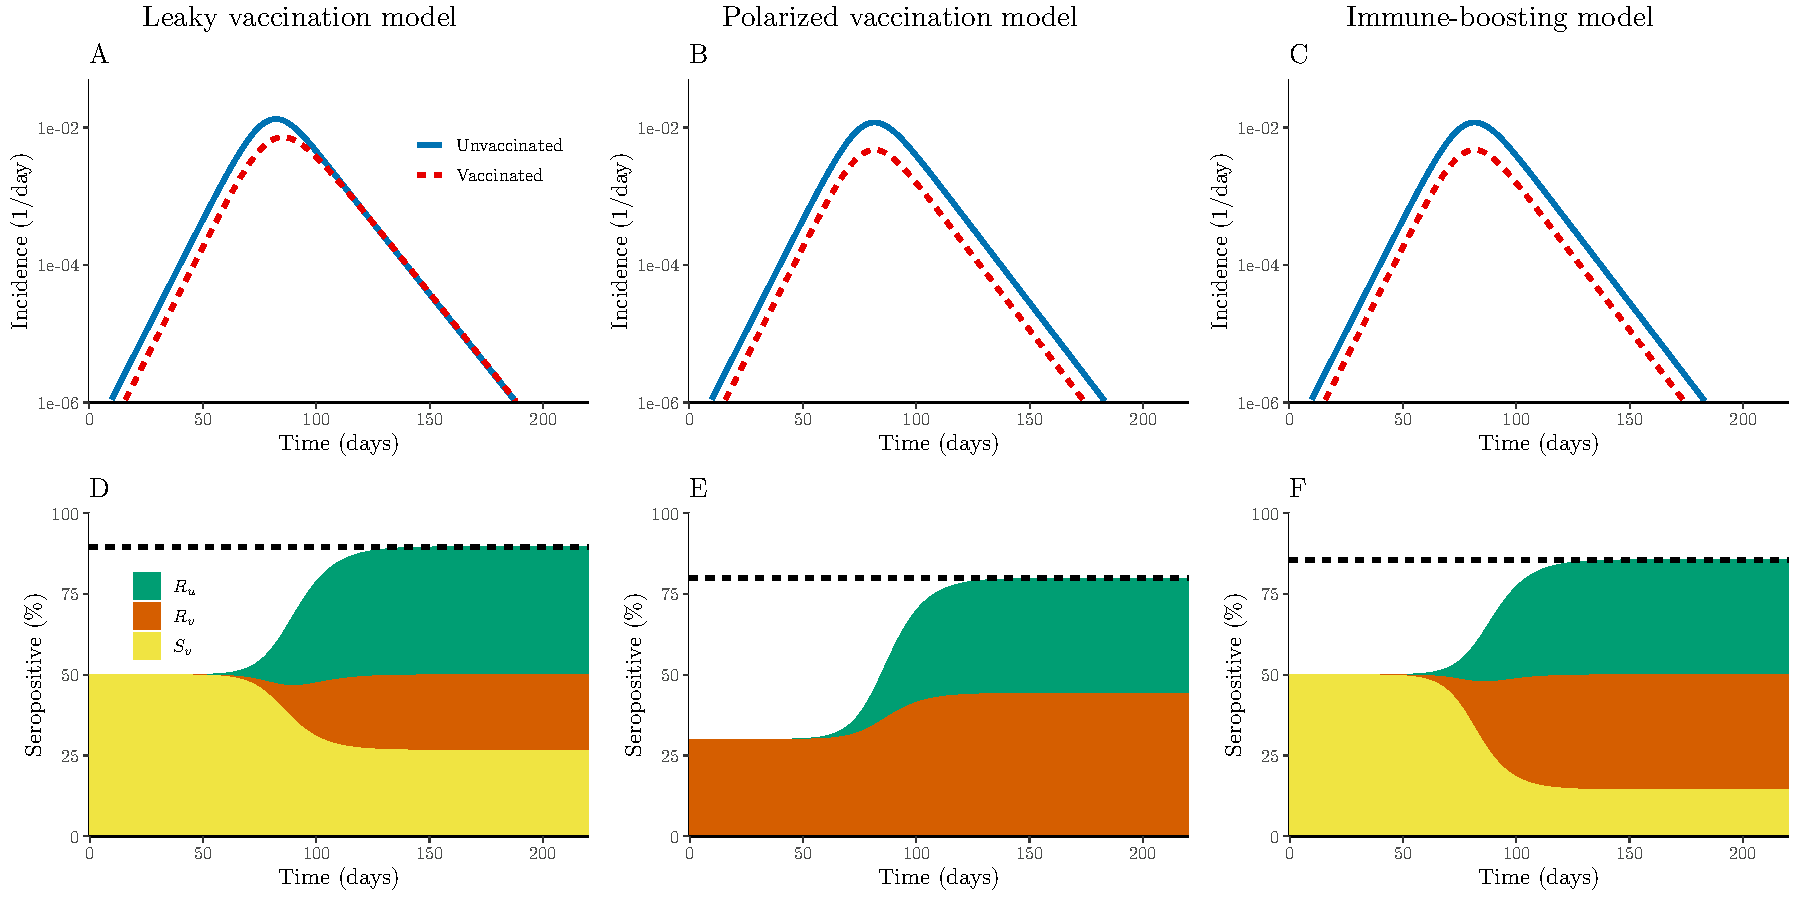
\includegraphics[width=\textwidth]{figure_simulation_compare.Rout.tikz.pdf}
\caption{
\textbf{Simulations of three different vaccination models.}
(A--C) Prevalence of infection among unvaccinated ($I_u$, blue solid) and vaccinated ($I_v$, orange dashed) individuals.
(D--F) Immune status over time (compartments $R_u$, $S_v$, and $R_v$).
The $S_v$ compartment is not included in the polarized vaccination model because it represents a set of individuals who have not retained any immunity from vaccination.
Simulations are performed assuming $\beta_u = \beta_v =0.5/\mathrm{day}$ for an average infectious periods of $1/\gamma=5~\mathrm{days}$.
We also assume that $\phi = 0.5$ proportion of individuals are vaccinated at the beginning of an epidemic with 60\% efficacy ($\VEP=\VEL=0.6$) and that vaccination does not continue during the outbreak ($\rho = 0$).
\label{fig:simulation}
}
\end{figure}

We then use the generalized vaccination model to further investigate how the final size of the an epidemic among vaccinated individuals depends on assumptions about vaccine-derived immunity across a wide range of assumptions about the basic reproduction number $\mathcal R_0$ and vaccine efficacy $\VE$ (\fref{sensitivity}).
In particular, we factor vaccine efficacy $\VE$ in terms of leaky vaccine efficacy \VEL\ and polarized vaccine efficacy \VEP; we consider an intermediate case, in which $\VEL = \VEP = 1 - \sqrt{1-\VE}$, as well as the extreme cases, in which case $\VEL = \VE$ or $\VEP = \VE$.
First, when $\VEL = \VE$, all vaccinated individuals have identical susceptibility;
in this case, increasing the amount of boosting $q$ reduces the final size as expected (see first column of \fref{sensitivity}).
We observe biggest effects of boosting at intermediate vaccine efficacy, $\VE$, and high basic reproduction number, $\mathcal R_0$ (see bottom left panel of \fref{sensitivity}).
When vaccine efficacy is too low (or too high), then boosting has negligible effects because virtually everyone (or virtually no one) gets infected.
As we increase $\mathcal R_0$, the leaky vaccination model predicts that all vaccinated individuals will eventually get infected.
On the other hand, the final size predicted by the immune boosting model cannot be greater than $1-\VE$.
As we increase \VEP\ (and decrease \VEL\ accordingly), the generalized vaccination model collapses to the polarized vaccination model, and the final size becomes insensitive to the boosting parameter $q$.

\begin{figure}[!th]
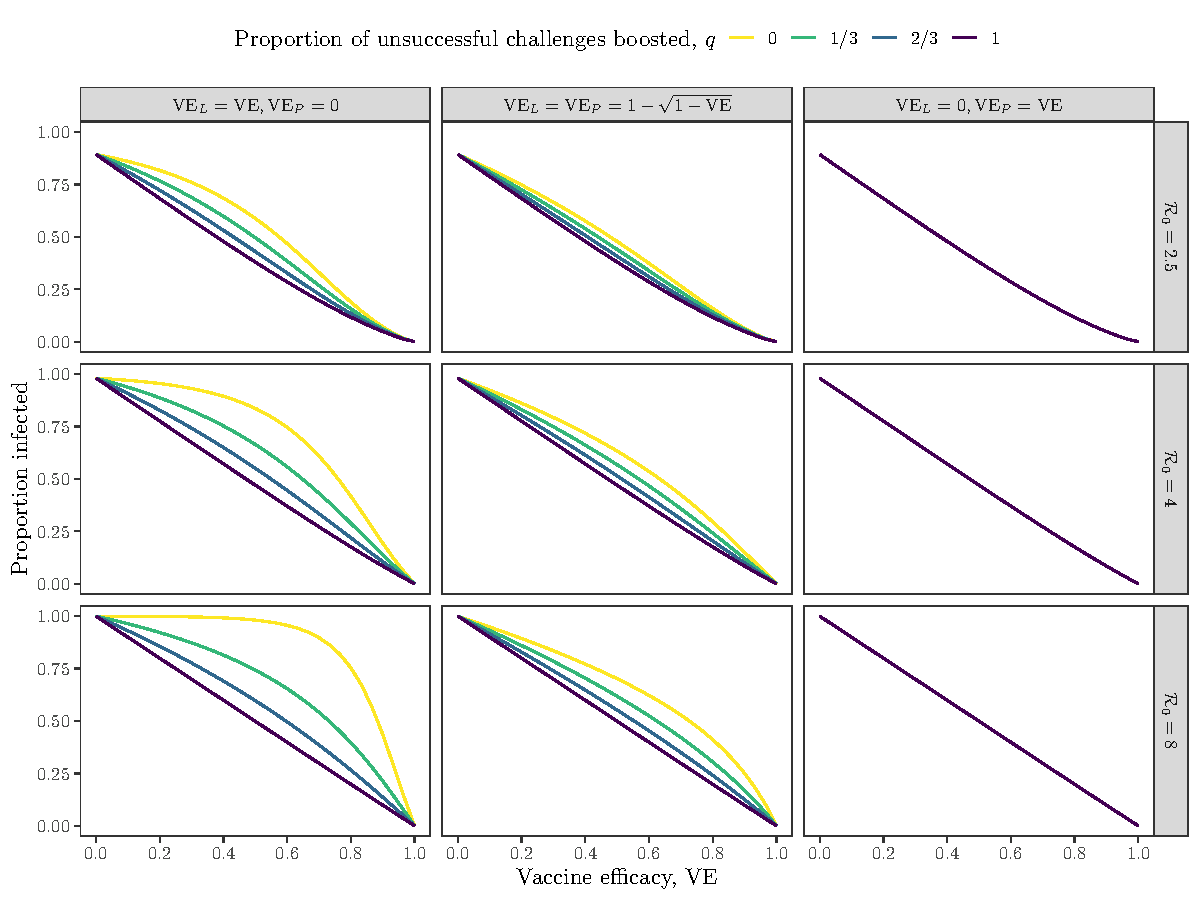
\includegraphics[width=\textwidth]{figure_simulation_generalized.Rout.vaccinated.tikz.pdf}
\caption{
\textbf{Sensitivity of the final size of an outbreak among vaccinated individuals to assumptions about vaccine-derived immunity}
Final size of an outbreak was calculated by simulating the generalized vaccination model for 220 days.
All other parameters are the same as in \fref{simulation}.
\label{fig:sensitivity}
}
\end{figure}

So far, we have limited our discussions to vaccine efficacy, which we defined as the proportion of people protected from their first challenge. 
We distinguish this from vaccine \textit{effectiveness}, which is measured empirically. 
Here, we compare two ways of estimating vaccine effectiveness: using cumulative incidence or instantaneous hazard.
Several factors can cause vaccine effectiveness to systematically differ from vaccine efficacy---in our case, the main reason is the fact that some vaccinated individuals may be challenged multiple times.

Cumulative incidence refers to the cumulative proportion of infections among unvaccinated and vaccinated individuals; 
this is typically used for measuring the vaccine effectiveness from real-life outbreaks \citep{farrington1993estimation}.
Since we are modeling a single epidemic without a loss of immunity or multiple infections, we consider the reduction in cumulative incidence throughout the entire epidemic.
To do so, we add two additional compartments, which keep track of cumulative incidence among unvaccinated $C_u$ and vaccinated $C_v$ individuals:
\begin{align}
\frac{\dd C_u}{\dd t} &= \lambda S_u\\
\frac{\dd C_v}{\dd t} &= (1-\VEL) \lambda S_v
\end{align}
Since we are neglecting vaccinations that occur during the outbreak ($\rho=0$, the cumulative proportion of infections among vaccinated $p_v(t)$ and unvaccinated $p_u(t)$ individuals can be expressed as:
\begin{align}
p_u(t) &= C_u(t)/S_u(0)\\
p_v(t) &= C_v(t)/S_v(0)
\end{align}
Then, the estimated vaccine effectiveness at time $t$ corresponds to:
\begin{equation}
1 - \frac{p_v(t)}{p_u(t)}.
\end{equation}

On the other hand, instantaneous hazard refers to the per-capita rate at which unvaccinated $h_u(t)$ and vaccinated $h_v(t)$ individuals get infected if they have not yet been infected yet.
These quantities can be calculated by diving the incidence of new infection by the number of uninfected individuals.
The per-capita rate of infection $h_v(t)$ among vaccinated individuals in then given by:
\begin{equation}
h_v(t) = \frac{(1-\VEL) \lambda(t) S_v(t)}{S_v(0) - C_v(t)},
\end{equation}
where $S_v(0) - C_v(t) \geq S_v(t)$ because vaccinated individuals can leave the $S_v(t)$ compartment via boosting;
in other words, we are assuming that boosting does not count as infection.
The per-capita rate of infection $h_u(t)$ among unvaccinated individuals is straightforward: 
\begin{equation}
h_u(t) = \frac{\lambda(t) S_u(t)}{S_u(t)} = \lambda(t).
\end{equation}
Then, the estimated reduction in hazard at time $t$ corresponds to:
\begin{equation}
1 - \frac{h_v(t)}{h_u(t)}.
\end{equation}

We compare two estimates of vaccine effectiveness across a wide range of assumptions about vaccine-derived immunity in \fref{efficacy}.
We assume 60\% efficacy throughout (therefore $\VE = 0.6$).
When all unsuccessful challenges result in immune boosting ($q=1$, immune boosting model in \fref{diagram}), the cumulative-incidence reduction always gives correct answers throughout the epidemic---since the susceptible pool among unvaccinated and vaccinated individuals is depleted at the same rate $\lambda$, the ratios of their proportions of cumulative infections remain constant.
Likewise, the cumulative-incidence reduction also give correct answers for the polarized vaccination model ($\VEL = 0$, $\VEP = \VE$).
However, when some challenges are not boosted ($q < 1$), using cumulative incidence underestimates the vaccine efficacy beyond the exponential growth phase.
This is because vaccinated individuals who have been exposed but are not boosted or infected still remain susceptible to future infections; 
larger final epidemic sizes predicted by these models (\fref{sensitivity}) then translate to a seemingly lower vaccine efficacy.

The hazard reduction gives correct answers for the leaky vaccine model (when $q=0$, $\VEL = \VE$, and $\VEP = 0$) because the ratios of force of infection that unvaccinated and vaccinated individuals experience are always constant.
However, the hazard reduction overestimates vaccine efficacy in the presence of immune boosting: since boosted individuals have not yet been infected, the susceptible pool in the vaccinated group appears to be bigger than it really is, causing the per-capita rate of infection to seem smaller.
Vaccine efficacy is also overestimated for polarized vaccination for similar reasons.

We note that both estimates give correct answers during the exponential growth phase, regardless of underlying assumptions about immunity.
More generally, we expect both estimates to give unbiased estimates as long as the depletion of susceptible pool is negligible among both vaccinated and unvaccinated individuals;
in trial settings, where incidence is relatively low, this assumption may hold.
But estimating vaccine effectiveness from real outbreaks is expected to be more difficult especially when the disease is spreading rapidly and causing susceptible depletion.

\begin{figure}[!th]
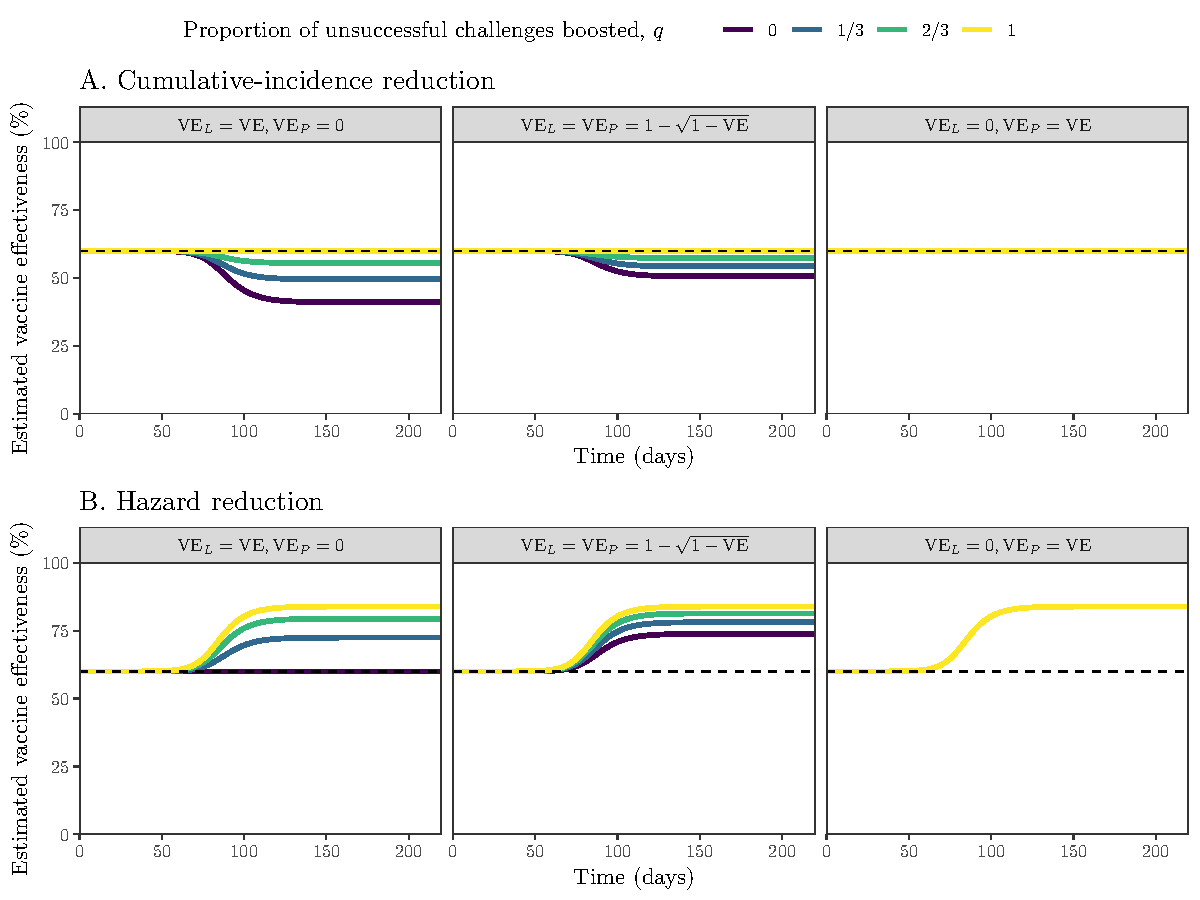
\includegraphics[width=\textwidth]{figure_simulation_efficacy.Rout.tikz.pdf}
\caption{
\textbf{Estimates of vaccine effectiveness using reduction in cumulative incidence (A) and hazard (B) over time.}
Vaccine effectiveness was calculated by simulating the generalized vaccination model for 220 days. 
Colored lines represent the estimated vaccine effectiveness.
Dashed lines represent the assumed vaccine efficacy.
We assume $\Ro = 2.5$ and a combined efficacy of $\VE = 0.6$ throughout. 
All other parameters are the same as in \fref{simulation}.
\label{fig:efficacy}
}
\end{figure}

\section*{Discussion}

Understanding the degree to which vaccination provides protection against infections is critical to predicting their population-level impact on epidemic dynamics.
Two models of vaccine-derived immunity have been previously proposed: leaky and polarized vaccination models.
The polarized model has been largely neglected in epidemiological modeling due to its apparently extreme assumption that a fraction of vaccinated individuals do not receive any protection. 
But the leaky vaccination model also makes an unrealistic assumption that vaccinated individuals who are exposed to infections can still remain susceptible, independent of previous exposures; 
a such assumption causes the leaky vaccination model to always predict a larger epidemic final size.
The differences in their epidemic dynamics can be understood by immune boosting: vaccinated individuals can attain protection without developing a transmissible infection, and therefore their infections are no longer independent of their previous exposures.
In particular, the immune boosting model predicts identical epidemic dynamics as the polarized vaccination model because the number of individuals who develop complete protection from polarization is equal to to the number of individuals who are boosted through exposure.

We also present a generalized vaccination model, which captures the dynamics of all three models.
Even though immune boosting and polarized vaccination models predict the same epidemic dynamics, they have different immune-status dynamics---these differences can be bridged by the generalized vaccination model.
The generalized vaccination model includes two additional parameters, which determine the amount of immune boosting and the proportion of individuals that remain partially susceptible after vaccination (rather than fully protected).
Using the generalized vaccination model, we show that the epidemic dynamics are most sensitive to the assumptions about vaccine-derived immunity at a intermediate vaccine efficacy.

Previous studies have tried to understand the differences between leaky and polarized vaccination models using arguments based on heterogeneity in susceptibility.
For example, leaky vaccination represents one extreme in which everyone has identical susceptibility;
polarized vaccination represents another extreme in which vaccinated individuals are either completely susceptible or not susceptible.
\cite{gomes2014missing} tried to reconcile these two assumptions by using a smooth distribution of susceptibility that changes from a delta distribution (leaky vaccination) to a polarized distribution;
however, they found that the predicted epidemic dynamics do not converge even though the distributions converge.
Our framework provides a simple explanations for these discrepancies:
regardless of the shape of the distribution of susceptibility, the leaky vaccination model always assumes that the infection events are independent of previous exposures.
On the other hand, the polarized distribution scenario no longer assumes independence because all exposures result in successful infections (for susceptible, vaccinated individuals).
In fact, the shape of the susceptibility distribution does not matter under immune boosting.
In Supplementary Materials, we provide a mathematical proof that the epidemic dynamics only depend on the mean susceptibility and are independent of the shape of the susceptibility distribution when immune boosting is included in the leaky vaccination model; we also present simulations to further illustrate the equivalence.
Therefore, we argue that neglecting immune boosting can lead to misleading conclusions about the effects of susceptibility heterogeneity in epidemic dynamics.\swp{maybe too strong?}

Finally, assumptions about vaccine-derived immunity also have important implications for estimating vaccine efficacy.
Vaccine efficacy can be estimated based on either the cumulative incidence or hazard rates.
The cumulative-incidence-based estimates give correct answers for polarized vaccination and immune boosting models,
whereas the hazard-based estimates give correct answers for the leaky vaccination model.
Neither methods give correct answers for intermediate cases in which there is partial polarization or boosting.
Nonetheless, both methods give correct estimates of vaccine efficacy for all vaccination models when susceptible depletion is negligible.
Therefore, vaccine efficacy and effectiveness estimates should be interpreted with care, especially when a large fraction of vaccinated individuals have been infected.

We rely on a simplifying assumption that natural infections (as well as polarized vaccination and immune boosting) provide complete protection against future infections.
In practice, both infection- and vaccine-derived immunity wanes over time for many pathogens \citep{heffernan2009implications,lewnard2018vaccine,perez2022}.
When immunity wanes, polarized vaccination and immune boosting models may not necessarily predict identical dynamics.
In particular, individuals who gain complete protection through polarized immunity immediately enter the $R_v$ compartment upon vaccination, whereas those who gain complete protection through immune boosting take longer to enter the $R_v$ compartment because they need to be exposed to infections.
These differences can translate to shorter delays between reinfection events for the polarized immunity model, which in turn can lead to dynamical differences at the population level.
There are also other complexities that need to be considered.
For example, individuals who are boosted after vaccination can have different immunity profiles compared to those who attained strong protection from vaccination alone.
These individuals also likely have different immunity profiles from those who have been infected but never been vaccinated.
These differences can also cause polarized vaccination and immune boosting models to behave differently.
Despite these limitations, immune boosting, which is often neglected in epidemic models of vaccination, is still expected to be an important mechanism for understanding dynamics of many pathogens.

We have provided a unifying framework for understanding the impact of vaccination on the spread of infectious disease.
\swp{concluding paragraph please...}

\pagebreak

\section*{Supplementary Text}

Here, we show that epidemic dynamics only depend on the mean susceptibility and are independent of the shape of the susceptibility distribution in the presence of immune boosting.
To do so, consider a immune boosting model that allows for heterogeneity in vaccine-derived immunity.
We assume that a vaccinated individual's susceptibility $0 \leq p \leq 1$ follows some distribution $f(p)$:
\begin{align}
\frac{\dd S_u}{\dd t} &= - \lambda(t) S_u - \rho S_u \\
\frac{\dd I_u}{\dd t} &= \lambda(t) S_u - \gamma_u I_u \\
\frac{\dd R_u}{\dd t} &= \gamma_u I_u \\
\frac{\partial S_v(p)}{\partial t} &= - \lambda(t) S_v(p) + f(p) \rho S_u  \\
\frac{\partial I_v(p)}{\partial t} &= p \lambda(t) S_v(p) - \gamma_v I_v(p) \\
\frac{\dd R_v}{\dd t} &= \int_0^1 \left[ (1-p) \lambda(t) S_v(p) + \gamma_v I_v(p) \right]\dd p
\end{align}
Due to immune boosting, $S_v(p)$ is always depleted at a per-capita rate of $\lambda(t)$ regardless of the values of $p$, meaning that the (normalized) distribution of $S_v(p)$ will always follow $f(p)$.
To obtain the dynamics of total prevalence $I_v = \int I_v(p) \dd p$, we can integrate $\partial I_v(p)/\partial t$ across $p$:
\begin{align}
\frac{\dd I_v}{\dd t} &=  \int_0^1\left[\frac{\partial I_v(p)}{\partial t}\right]\dd p\\
&= \int_0^1\left[p \lambda(t) S_v(p) - \gamma_v I_v(p)\right]\dd p\\
&= \int_0^1\left[p f(p) \lambda(t) S_v - \gamma_v I_v(p)\right]\dd p\\
&= \bar{p} \lambda(t) S_v - \gamma_v I_v,
\end{align}
where $\bar{p}$ represents the mean of the distribution $f(p)$, and $S_v = \int S_v(p) \dd p$ represents the proportion of total susceptible, vaccinated individuals.
Therefore, the dynamics of total prevalence $I_v$ depends only on the mean susceptibility $\bar{p}$ and not on the shape of the distribution $f(p)$ under immune boosting.

\pagebreak

\bibliography{immune_boosting}

\end{document}
